\documentclass[12pt]{article}

% BASIC PACKAGES
\usepackage[utf8]{inputenc}
\usepackage[english]{babel}
\usepackage{csquotes}
\usepackage{mathtools}
\usepackage{hyperref}
\usepackage{geometry}
\usepackage{amsfonts}
\usepackage{amsmath}
\usepackage{amssymb}
\usepackage{graphicx}
\usepackage[small,bf,center]{caption}
\usepackage{subfig}
\usepackage{setspace}
\usepackage{float}
\usepackage[section]{placeins} % for \FloatBarrier

% XXXXXX PACKAGES
\usepackage{indentfirst}

\newtheorem{prop}{Proposition}

\begin{document}

% FIRST PAGE -------------------------------------------------------------------

\title{\vspace{-3cm}
      Expecting to get it: \\ An endowment effect for information
      }

\author{Tabaré Capitán
          \thanks{Corresponding author: Tabare.Capitan@gmail.com. For their useful comments, we thank Hunt Allcott, James Heckman, Stephan Kroll, John List, Daniel Millinet, and Stephen Newbold. We also thank participants in seminars at UA Anchorage, the University of Chicago, Colorado State University, the 2019 North American Economic Science Association meetings, and the 2020 Bogotá Experimental Economics Conference. Financial support from USDA/NIFA (grant number 2016-09907) is gratefully acknowledged. The collection of data for this study was approved by the IRB at University of Wyoming.}
        \and
        Linda Thunström
        \and
        Klaas van ‘t Veld
          \\ \small{Department of Economics, University of Wyoming}
        \and
        Jonas Nordström
          \\ \small{Lund University and University of Copenhagen}
        }

\maketitle

\thispagestyle{empty}   % Suppress page number (must be under \maketitle)

\begin{abstract}

\noindent
PENDING PENDING PENDING PENDING PENDING PENDING PENDING PENDING PENDING PENDING PENDING PENDING PENDING PENDING PENDING PENDING PENDING PENDING PENDING PENDING PENDING PENDING PENDING PENDING PENDING PENDING PENDING PENDING PENDING PENDING PENDING PENDING PENDING PENDING PENDING PENDING PENDING PENDING PENDING PENDING PENDING PENDING PENDING PENDING PENDING PENDING
\\
\textit{Keywords:} expectations, reference-dependent preferences, preferences for information, information avoidance.
\\
\textit{JEL classification:} D01, D80, D83, D84, D91, C91.

\end{abstract}

\clearpage

\pagenumbering{arabic} % Start numbering in page 2 from #1

% INTRODUCTION -----------------------------------------------------------------
\section{Introduction}

Ana and Beto, separately, have decided to go to a café to eat a chocolate cake, and they are both equally concerned about their calorie intake. While they share the same belief about the calorie content of the cake, Ana expects the café to have calorie information on the menu and Beto does not. In this paper we show, both theoretically and empirically, that Ana’s expectation makes the information more valuable to her than to Beto.  In other words, an endowment effect for information arises from the very expectation of getting the information. We are not aware of previous work in which this endowment effect has been identified, let alone tested.\footnote{However, [CITE CAWLEY2020] provide suggestive evidence in a study in which participants with high exposure to calorie information were more supportive of calorie labels.}

The endowment effect we observe is closely related to the endowment effect for risk predicted by the theory of [CITE KR07] and tested by [CITE SPRENGER15]. Their endowment effect for risk arises because those expecting to face risk (a non-degenerate lottery over consumption outcomes) are more tolerant to risk than those expecting to face a certain outcome. In our case, expecting to receive information is akin to expecting to face risk (a non-degenerate lottery defined by the prior distribution of beliefs), whereas \emph{not} expecting to receive information is akin to expecting a certain outcome (the mathematical expectation of the prior distribution of beliefs).\footnote{[CITE KR09] develop another theory of expectations-based reference-dependent preferences\textemdash\emph{news utility}\textemdash that might seem closer to our work. However, their \emph{news utility} theory is about reference-dependence with respect to the \emph{content} of the information (i.e., what you might find out). Instead, the endowment effect for information arises from reference-dependence with respect to information \emph{delivery} (i.e., whether you find out), regardless of the content.}

The parallel to an endowment effect for risk is not perfect, however. Because the role of information in decision making goes beyond mere updating of beliefs, preferences for risk are not the same as preferences for information. Instrumental information can be used to adjust behavior (e.g., calorie information can induce Ana or Beto to eat less or more of their cake, or exercise more or less strenuously afterwards), and even non-instrumental information can spark curiosity ([CITE LOEWENSTEIN94]; [CITE TAROTSUSTEIN2020]).

The endowment effect for information that we derive fits in the theoretical literature on expectations-based reference-dependent preferences ([CITE ERICSONFUSTER14;[CITE ODONOGHUESPRENGER18]]).\footnote{[CITE SPRENGER15] reviews the related empirical literature, concluding that \enquote{Though both positive and negative results have been documented, an account of the literature would indicate some promise for the relevance of expectations in rationalizing reference-dependent behavior} (p1458).} In this literature, utility is separated into intrinsic utility (i.e., utility from outcomes) and gain-loss utility (i.e., utility from comparing outcomes to a referent). While the intrinsic utility is typically modeled in the same way across different theories, the specification of the gain-loss utility differs between the two leading theoretical approaches. The Disappointment Aversion approach ([CITE BELL85]; [CITE LOOMESSUGDEN86];[CITE GUL91]) collapses the reference lottery into a single value and measures the gain-loss utility relative to that value. In contrast, the  Kőszegi and Rabin approach ([CITE KR06]; [CITE KR97]) measures the gain-loss utility from every element of the outcome lottery relative to each element of the reference lottery separately, and then aggregates these gain-loss utilities to a single value.\footnote{The distinction between these two theoretical approaches is consequential only when the referent is stochastic, i.e., a reference lottery.}  In this paper, we show that both approaches predict an endowment effect for instrumental information, but only the Kőszegi and Rabin approach predicts an endowment effect for non-instrumental information.

We find evidence consistent with an endowment effect for information in a two-stage laboratory experiment, in which we offer participants a free cake and manipulate their expectations about whether they will get information about the cake’s calorie content. The idea of manipulating expectations to investigate the endowment effect builds on [CITE KR06] definition of a person’s referent as not the status quo, but rather \enquote{the \emph{expectations} a person held in the \emph{recent} past}, or more specifically \enquote{her probabilistic beliefs about the relevant consumption outcome held between the time she first focused on the decision determining the outcome and shortly before consumption occurs} (p.1141). They note also that the status quo can be viewed as a special case of this more general definition: in most experiments that treat the status quo as the referent, subjects plausibly expect the status quo to continue in future.

In the first stage, we vary participants’ \emph{experience} with calorie information in order to vary their sense of endowment. All participants are asked to choose their preferred dessert from eleven consecutive different menus, but those menus show calorie information for only half of the participants, and no calorie information for the other half. This priming manipulation is motivated by [CITE KR06]'s rationalization of [CITE LIST03]'s empirical finding that market experience reduces the (standard) endowment effect. The argument is that, because experienced traders are more likely to expect to trade their acquisitions, the endowment effect for them is smaller. More specifically, because experienced traders are less likely to extrapolate the status quo of having owned an item in the recent past to an expectation of retaining the item in the future, they experience less loss aversion when parting with the item through trading it away. As a result, they behave more like they would if they never owned the item in the first place, and in that sense exhibit less of an endowment effect.

% THE ARGUMENT BELOW IS HARD TO FOLLOW BECAUSE WE HAVE NOT SAID THAT THERE IS A SECOND MANIPULATION

Our manipulation applies the argument in the opposite direction. Whereas List’s experienced traders expected to \emph{give up} items, through their frequent exposure to trading, our experienced participants should expect to \emph{gain} information, through their frequent exposure to seeing it on menus. Experienced participants, we therefore predict, should be less likely to extrapolate the status quo of \emph{not} having information to an expectation of not getting it in future, and thus experience \emph{more} loss aversion when giving up the information. As a result, they will behave more like they would if they felt endowed with the information in the first place, and in that sense exhibit less of an endowment effect.\footnote{Note that the endowment \enquote{effect} is defined as a difference in behavior (e.g., willingness to trade a mug for a pen) depending on one’s sense of endowment. List’s experienced traders behaved similarly whether or not they were endowed with an item, thus exhibiting no endowment effect. We predict that experienced participants will behave similarly whether or not they were endowed with information, thus again exhibiting no endowment effect.}

In the second stage, we vary participants' \emph{first-focus} on calorie information to vary their sense of endowment. All participants are asked if they want to learn the calorie content of desserts on a menu, one of which, a cake, is marked as theirs to receive. For half of the participants, the menu includes a calorie-information column with the actual calorie numbers \enquote{temporarily} \emph{xxx}-ed out; for the other half, the menu shows nothing calorie-related.

This is the key manipulation of our experiment. It builds on the first-focus intuition implied by [CITE KR06] above-mentioned definition of the referent, which [CITE SPRENGER15] also exploits to test the endowment effect for risk.\footnote{Sprenger notes that the intuition is \enquote{in line with the psychological literature on \enquote{cognitive reference points} (Rosch 1974) and decision anchoring} (p.1462), which has shown referents to be susceptible to experimental variation.} Specifically, the \emph{xxx}-ed out calorie column on the first group's menu is intended to make participants focus first on getting calorie information when considering their choice whether to actually see it, and in that sense feel \emph{endowed} with the information. Conversely, the absence of any calorie-related information on the second group's menu is intended to make participants focus first on not getting information when considering the same choice, and in that sense feel \emph{not endowed} with the information.\footnote{Although we label our participants as \emph{endowed} or \emph{not endowed}, we do not claim that our manipulation \emph{fully} sets the referent. Instead, our key experimental manipulation varies the \emph{degree} to which participants feel endowed with the information. A more precise way to label our participats, used by [CITE HEFFETZLIST14], would be to use \emph{more endowed} and \emph{less endowed}. Nevertheless, we favor our labels to be consistent with the language typically used in the literature of the endowment effect.}

Our results support the existence of an endowment effect for information, in line with our theoretical prediction: among participants not primed in the first stage to expect calorie information, those endowed with information in the second stage asked to keep the information significantly more often than non-endowed participants asked to add it. Moreover, consistent with the argument that experience with information matters, this endowment effect was much weaker, and not statistically significant, for participants primed in the first stage to expect information.

% BEGING WORKING AREA \\\\\\\\\\\\\\\\\\\\\\\\\\\\\\\\\\\\\\\\\\\\\\\\\\\\\\\\\\

\textbf{PENDING [See Klaas' comments]}

% END WORKING AREA \\\\\\\\\\\\\\\\\\\\\\\\\\\\\\\\\\\\\\\\\\\\\\\\\\\\\\\\\\\\\

% THEORY -----------------------------------------------------------------------
\section{Theory: Disappointment Aversion and the Kőszegi and Rabin approach}

We model information preferences\textemdash preferences for taking or avoiding information\textemdash by applying and extending two theoretical approaches to modeling expectations-based reference-dependent preferences. One is the Disappointment Aversion (hereafter DA) approach pioneered by [CITE BELL85], with later contributions by [CITE LOOMESSUGDEN86] and [CITE GUL91]; the other is the Kőszegi and Rabin (hereafter KR) approach developed by Kőszegi and Rabin ([CITE KR06] [CITE KR07]). In our exposition, we follow the notation of [CITE ODONOGHUESPRENGER18] to discuss both approaches in a unified framework.

Formally, both approaches define the utility from a lottery of outcomes $L \equiv (x_1,p_1;x_2,p_2;...;x_N,p_N)$ given a reference lottery $R \equiv (r_1,q_1;r_2,q_2;...;r_M,q_M)$ as
\begin{equation*}
  U(L|R) \equiv \sum_{n=1}^{N} p_n[u(x_n)+v(x_n|R)],
\end{equation*}
where $u(x_n)$ is the intrinsic utility from lottery outcome $x_n$ and $v(x_n|R)$ is the gain-loss utility associated with that outcome. That is, $U(L|R)$ is the expected sum of intrinsic and gain-loss utility from each outcome of $L$.

The DA approach specifies the gain-loss utility from a specific outcome $x_n$ (from the lottery $L$) as
\begin{equation*}
  v(x_n|R) \equiv \mu (u(x_n)-\sum_{m=1}^M q_mu(r_m)),
\end{equation*}
i.e., as involving a comparison of the intrinsic utility of $x_n$ to the expected intrinsic utility from the reference lottery $R$. The gain-loss utility function $\mu(\cdot)$ is thereby specified as the piece-wise linear function
\begin{equation*}
  \mu(z)=
  \begin{cases}
    z          & \text{if } z \geq 0 \\
    \lambda z  & \text{if } z < 0 ,
  \end{cases}
\end{equation*}
where $\lambda>1$ (implying loss aversion). That is, if $u(x_n)$ is greater than $E[u(r_m)]$, this gives rise to gain utility $u(x_n)-E[u(r_m)]$, but if $u(x_n)$ is less than $E[u(r_m)]$, it gives rise to larger (in absolute terms) loss utility $\lambda(u(x_n)-E[u(r_m)])$.

In contrast, the KR approach specifies
\begin{equation*}
  v(x_n|R) \equiv \sum_{m=1}^M q_m \mu (u(x_n)-u(r_m));
\end{equation*}
that is, each outcome $x_n$ (from lottery $L$) is compared \emph{separately} to each individual outcome $r_m$ of the reference lottery $R$, giving rise (again with the same piece-wise linear gain-loss utility function) to gain utility $u(x_n)-u(r_m)$ if $u(x_n) \geq u(r_m)$ and to loss utility $\lambda [u(x_n)-u(r_m)]$ if $u(x_n)<u(r_m)$. The overall gain-loss utility $v(x_n|R)$ is the sum of all those separate gain and loss utility components, weighted by the probability $q_m$ of each outcome in $R$ that $x_n$ is compared to.

To make things more concrete and discuss the model in the context of preferences for information, consider our two cake eaters, Ana and Beto.\footnote{We emphasize that, in our example, Ana (who expects to receive information) and Beto (who expects not to receive information) are essentially the same person, except for their differing expectations.} Ana and Beto know that it is equally probable that the cake they are about to eat is either low- or high-calorie, and because they are both equally concerned about their calorie intake, their intrinsic utility of eating a high-calorie cake is \emph{low} ($l$), and their intrinsic utility of eating a low-calorie cake is \emph{high} ($h$). Furthermore, they do not anticipate being able to tell the cake’s calorie content from eating it, and, for now, they do not anticipate adjusting their behavior in response to the calorie information (i.e., the information is non-instrumental). Therefore, if they do not receive information about the calorie content of the cake, they will perceive eating the cake as yielding intrinsic utility $0.5h+0.5l$ (i.e., the probability weighted average of their utility in the low- and high-calorie states of the world).

Written in terms of lotteries, and for simplicity equating lottery outcomes with their induced utilities (i.e., skipping the intermediate step of mapping calories to intrinsic utilities), we can represent their situation if they currently do not know the cake's calorie content but will find out, as facing the lottery $L^i$ (superscript $i$ for \emph{informed}) equal to $(x_1=h,p=0.5;x_2=l,p_2=0.5)$. If they will \emph{not} find out, however, then they face the degenerate lottery $L^u$ (superscript $u$ for \emph{uninformed}) equal to $(x=0.5h+0.5l,p=1)$.

If their utility is reference-dependent, then their evaluation of these lotteries will depend on whether they \emph{expect} to be informed (i.e., see calorie information in the menu). For Ana, who expects to be informed, we can represent this as starting out with reference lottery $R^i=(r_1=h,q_1=0.5;r_2=l,q_2=0.5)$; for Beto, who expects not to be informed, we can represent this as starting with degenerate reference lottery $R^u=(r=0.5h+0.5l,q=1)$. Thus, there are four possible utilities:
\begin{itemize}
	\item $U(L^i|R^i)$ from expecting to be informed and getting information,
	\item $U(L^u|R^i)$ from expecting to be informed and not getting information,
	\item $U(L^i|R^u)$ from expecting to be uninformed and getting information, and
  \item $U(L^u|R^u)$ from expecting to be uninformed and not getting information.
\end{itemize}

An endowment effect is predicted if receiving the information is more valuable to a person who expects to receive it (like Ana) than to a person who does not expect to receive it (like Beto):\footnote{[CITE SPRENGER15] emphasizes that the KR endowment effect for risk that he tests for \enquote{should be thought of as distinct from the standard endowment effect literature documenting exchange anomalies as discrepancies between WTP and WTA for the same object. The KR endowment effect for risk is a risk preference discrepancy between risk taking when the referent is certain and risk taking when the referent is stochastic.} (p.1458) Similarly, in our context, the endowment effect for information is an information preference discrepancy between information seeking when the referent is certain (i.e., an agent does not expect to receive information, making the referent a degenerate lottery) and information seeking when the referent is stochastic (i.e., the agent expects to receive information, making the referent a non-degenerate lottery).}
\begin{equation}
  U(L^i|R^i)-U(L^u|R^i)>U(L^i|R^u)-U(L^u|R^u).
  \label{eq:endowmentEffect}
\end{equation}

Below we discuss four results regarding the existence of an endowment effect for information under the DA or the KR approach when information is either non-instrumental or instrumental. \textbf{SEE APPENDIX FOR PROOFS.}

\begin{prop}
  Assume reference-dependent utility following the DA approach, with a piece-wise linear gain-loss utility function and non-instrumental information. For any lottery $L$, $U(L^i|R^i)-U(L^u|R^i)=U(L^i|R^u)-U(L^u|R^u)$. Therefore, no endowment effect is predicted.
  \label{prop:nonInstrumental-DA}
\end{prop}

\begin{figure}[ht]
  \caption{Value of information under the DA approach, with non-instrumental information.}\label{fig:nonInstrumental-DA}
  \begin{center}
  {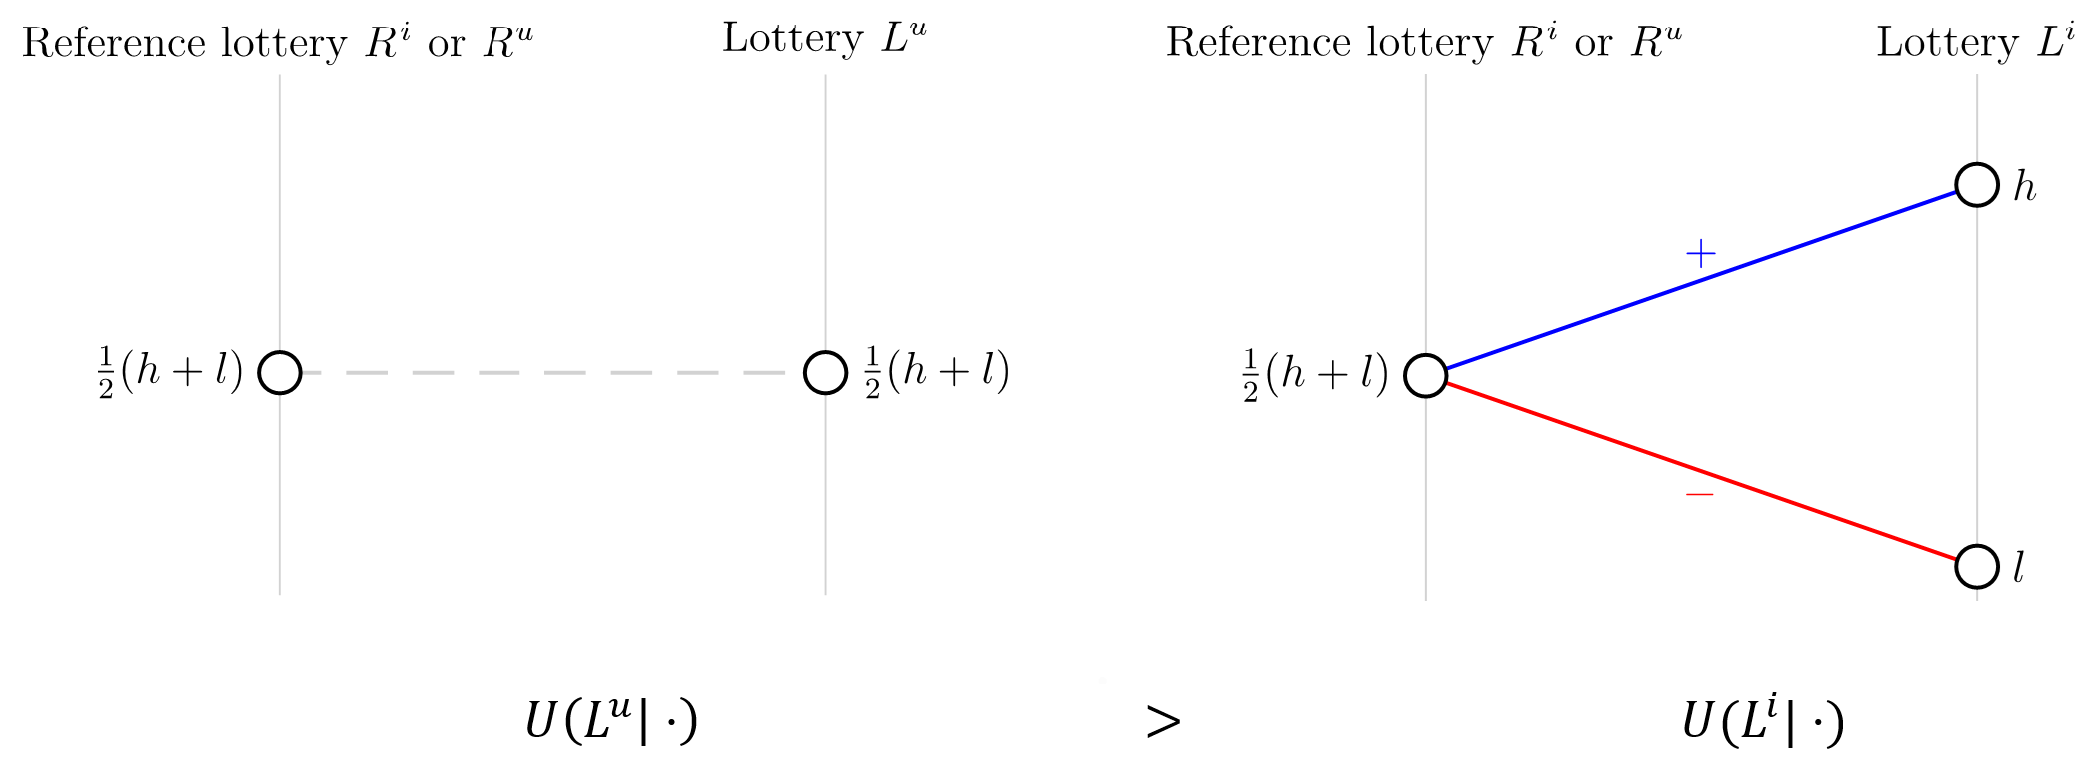
\includegraphics[width=1\textwidth]{./figures/theory_fig1.png}}
  \end{center}
\end{figure}

Because under the DA approach the reference lottery collapses to its expectation before evaluating gain-loss utility, and given that both referents $R^i$ an $R^u$ have the same expectation $E[R^i]=E[R^u]=0.5(h+l)$, the difference $U(L^i|\cdot)-U(L^u|\cdot)$ is the same regardless of wheter a person expects to receive information or not. Specifically, as illustrated in Figure \ref{fig:nonInstrumental-DA}, relative to not getting information (illustrated in the left panel), getting information (illustrated in the right panel) involves a gain of $h-0.5(h+l)=0.5(h-l)$ with probability one-half and a utility loss of $l-0.5(h+l)=-0.5(h-l)$ with probability one half. Because of loss aversion, however, the utility loss receives additional weight $\lambda>1$, implying that $U(L^i|\cdot)-U(L^u|\cdot)=-0.25(\lambda-1)(h-l)<0$. In other words, the value of information is equally negative, regardless of expectations.

\FloatBarrier

\begin{prop}
  Assume reference-dependent utility following the KR approach, with a piece-wise linear gain-loss utility function and non-instrumental information. For any lottery $L$, $U(L^i|R^i)-U(L^u|R^i)>(L^i|R^u)-U(L^u|R^u)$. Therefore, an endowment effect is predicted.
  \label{prop:nonInstrumental-KR}
\end{prop}

\begin{figure}[ht]
  \caption{Value of information under the KR approach, with non-instrumental information.}\label{fig:nonInstrumental-KR}
  \begin{center}
  {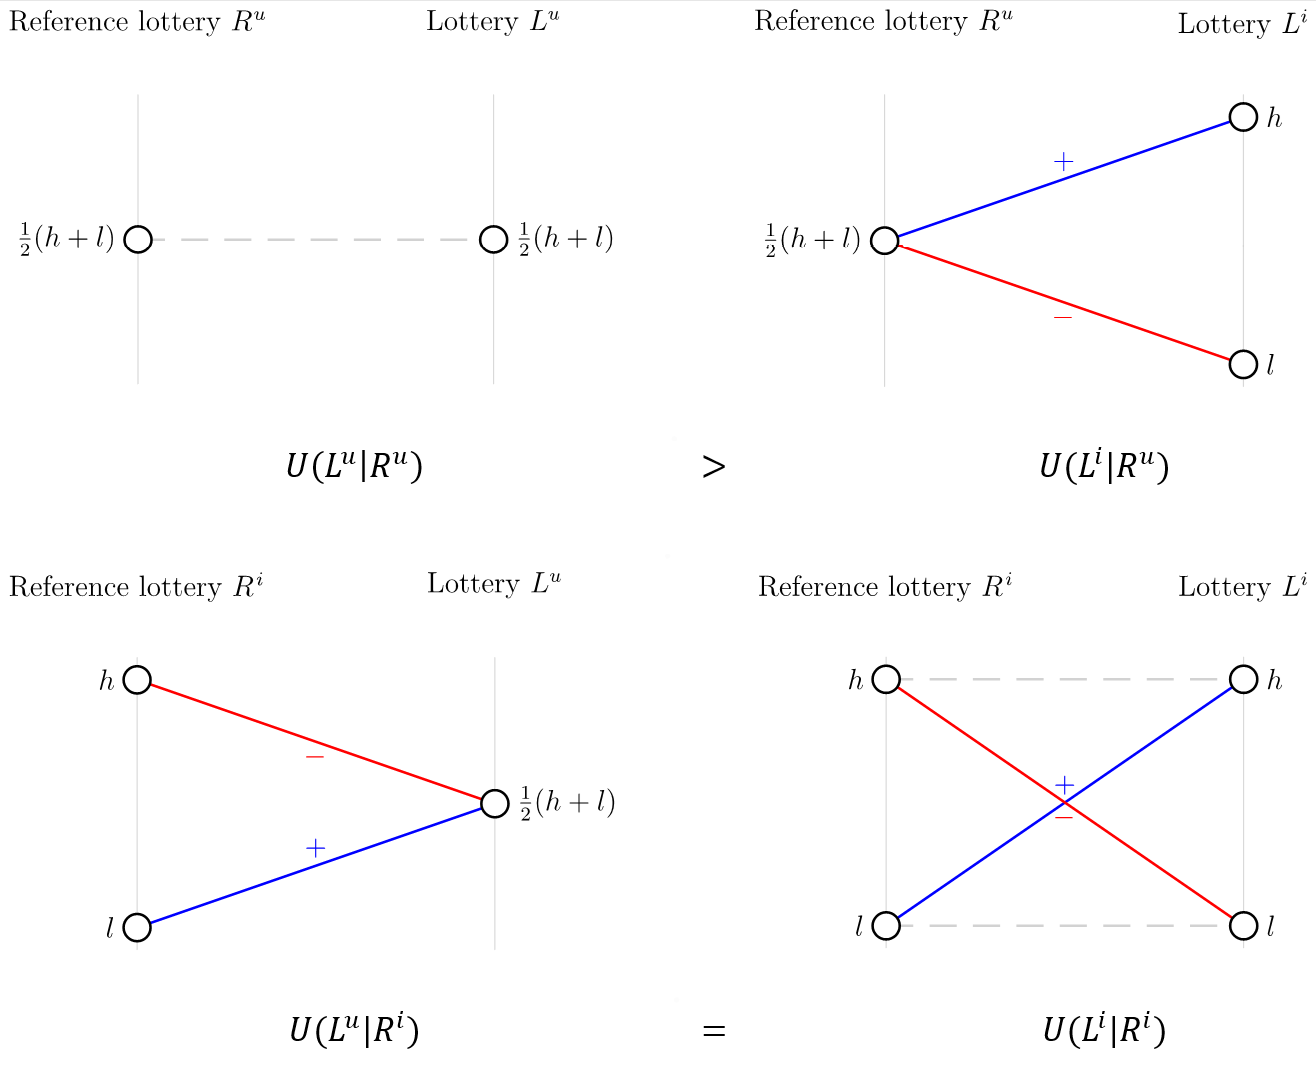
\includegraphics[width=1\textwidth]{./figures/theory_fig2.png}}
  \end{center}
\end{figure}

Figure \ref{fig:nonInstrumental-KR} illustrates how the endowment effect for information arises under the KR approach. Since all four possible outcomes yield the same intrinsic utility $0.5(h+l)$, the endowment effect is driven by differences in gain-loss utility depending on expectations.

If information is not expected (illustrated in the top panels), getting it results in the same net utility loss $U(L^i|R^u)-U(L^u|R^u)=-0.25(\lambda-1)(h-l)<0$ as under the DA approach. In other words, Beto's value of information is negative\textemdash{he is information averse}.

If information is expected (illustrated in the bottom panels), then not getting it (the bottom-left panel) involves a utility gain of $0.5(h+l)-l=0.5(h-l)$ and a loss $0.5(h+l)-h=-0.5(h-l)$, each weighted by probability one-half. Because the loss receives additional weight $\lambda>1$, the net gain-loss utility is $-0.25(\lambda-1)(h-l)<0$. But\textemdash and this is key\textemdash getting information that is expected (the bottom-right panel) involves a \emph{twice larger} utility gain of $(h-l)$ and loss of $-(h-l)$, each weighted \emph{twice smaller} probability one-quarter, before applying outcomes $l$ in both. On net, then, the gain-loss utility ends up being the same $-0.25(\lambda-1)(h-l)<0$, implying that $U(L^i|R^i)-U(L^u|R^i)=0$. In other words, Ana's value of information is zero\textemdash{she is information neutral}.

Comparing Ana's and Beto's value of information, we find an endowment effect:
\begin{equation*}
  [U(L^i|R^i)-U(L^u|R^i)]-[U(L^i|R^u)-U(L^u|R^u)]=0.25(\lambda-1)(h-l)>0.
\end{equation*}
Note that, at least for non-instrumental information, the endowment effect does not make Ana value information more positively. Rather, it makes her value information \emph{less negatively}: she becomes information neutral rather than information averse.

Proposition \ref{prop:nonInstrumental-KR} is closely related to the prediction of an endowment effect for risk in [CITE KR07]. In fact, we have treated information in a way that parallels the way monetary risk is treated in their model: expecting to receive information is akin to having a stochastic referent, and expecting not to receive information is akin to having a non-stochastic referent.

The parallel extends further to Kőszegi and Rabin’s characterization of the psychology underlying their endowment effect for risk. They remark that their predictions crucially \enquote{do \emph{not} imply that a person is unbothered by risk she expects or faces, even if it does make her less risk averse.} Rather, a decisionmaker who had been expecting risk, or is already facing risk, \enquote{is already exposed to stochastic utility-decreasing sensations of loss, so taking additional risk does not add so much exposure to losses} (p. 1054). In our context, the endowment effect for information may arise similarly because those who expect information have already built utility-decreasing sensations of loss into their expected utility. In other words, those who expect information are more willing to get it, because they are already exposed to the potential pain of disappointment outweighing the potential joy of pleasant surprise.

\FloatBarrier

Up until this point, we have assumed that information is non-instrumental. Because of this, information has served a role only in determining whether a lottery is degenerate or not, making our formalism so far indistinguishable from formalisms analyzing monetary risk. However, information can serve the additional role of allowing people to adjust current and future choices in response to it. For example, if Ana or Beto learn the calorie content of the cake, they can decide to eat less or more of  it, or adjust how much they subsequently exercise.

Suppose for simplicity that these adjustments would increase their utility by the same amount $\Delta > 0$ in both states of the world, and define $h^* \equiv h+\Delta$ and $l^* \equiv l+\Delta$. Thus, given her expectation of learning the calorie content of the cake, Ana expects to be able to make adjustments and get intrinsic utility $0.5(h^*+l^*)$. Assuming adjustments are not so large to turn bad news into good news, which requires $\Delta <0.5(h-l)$, we then have propositions \ref{prop:instrumental-DA} and \ref{prop:instrumental-KR}.

\begin{prop}
  Assume reference-dependent utility following the DA approach, with a piece-wise linear gain-loss utility function and instrumental information. For any lottery $L$, $U(L^i|R^i)-U(L^u|R^i)>(L^i|R^u)-U(L^u|R^u)$. Therefore, an endowment effect is predicted.
  \label{prop:instrumental-DA}
\end{prop}

\begin{figure}[ht]
  \caption{Value of information under the DA approach, with instrumental information.}\label{fig:instrumental-DA}
  \begin{center}
  {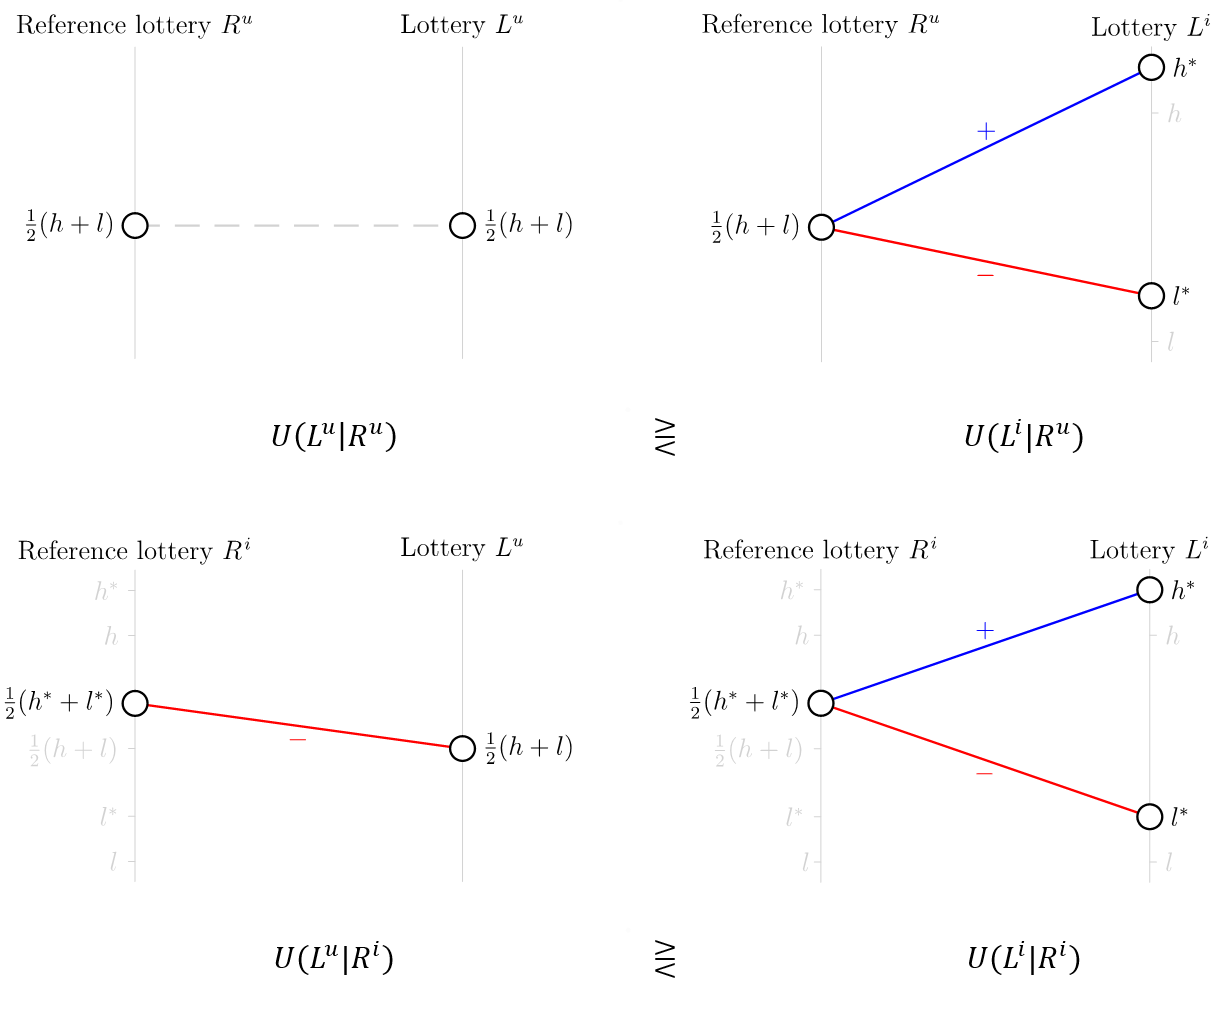
\includegraphics[width=1\textwidth]{./figures/theory_fig3.png}}
  \end{center}
\end{figure}

Figure \ref{fig:instrumental-DA} illustrates how the endowment effect now arises under the DA approach as well. The ability to make behavioral adjustments adds $0.5 \Delta + 0.5 \Delta = \Delta$ to the intrinsic utility of getting information, regardless of expectations. If information is unexpected (illustrated in the top panels), however, then the gained ability to adjust enhances the gain from the good outcome and mitigates the loss from the bad outcome, thereby adding $0.5 \Delta + 0.5 \lambda \Delta = 0.5 (1 + \lambda) \Delta$ to gain-loss utility. The overall value of unexpected information becomes
\begin{equation*}
  U(L^i|R^u)-U(L^u|R^u)=-0.25(\lambda-1)(h-l)+\Delta +0.5(1+\lambda)\Delta,
\end{equation*}
which for large enough $\Delta$ may be positive.

If information is expected (illustrated in the botoom panels), then the \emph{forgone} ability to adjust gives rise to loss utility $-0.5\Delta - 0.5 \lambda \Delta = -\lambda \Delta$ from \emph{not} getting information (the bottom-ledt panel). Because both the $R^i$ and $L^i$ lotteries shift up by the same amount $\Delta$, however, gain-loss utility from getting information (the bottom-right panel) is unchanged. The overall value of expected information therefore becomes
\begin{equation*}
  U(L^i|R^i)-U(L^u|R^i)=-0.25(\lambda-1)(h-l)+\lambda +\lambda \Delta
\end{equation*}

Moreover, because $\lambda>1$ implies that $\lambda \Delta > 0.5(1+\lambda)\Delta$, the value of expected information now exceeds that of unexpected information, implying an endowment effect. In short, the ability to adjust enhances the value of expected information by an avoided sure loss of $\lambda \Delta$, but the value of unenxpected information by an avoided loss of $\lambda \Delta$ only with probability one-half, together with a gain of $\Delta$ with probability one-half. If losses outweigh gains, the former effect dominates.

\FloatBarrier

\begin{prop}
  Assume reference-dependent utility following the KR approach, with a piece-wise linear gain-loss utility function and instrumental information. For any lottery $L$, $U(L^i|R^i)-U(L^u|R^i)>(L^i|R^u)-U(L^u|R^u)$. Therefore, an endowment effect is predicted.
  \label{prop:instrumental-KR}
\end{prop}

\begin{figure}[ht]
  \caption{Value of information under the DA approach, with instrumental information.}\label{fig:instrumental-KR}
  \begin{center}
  {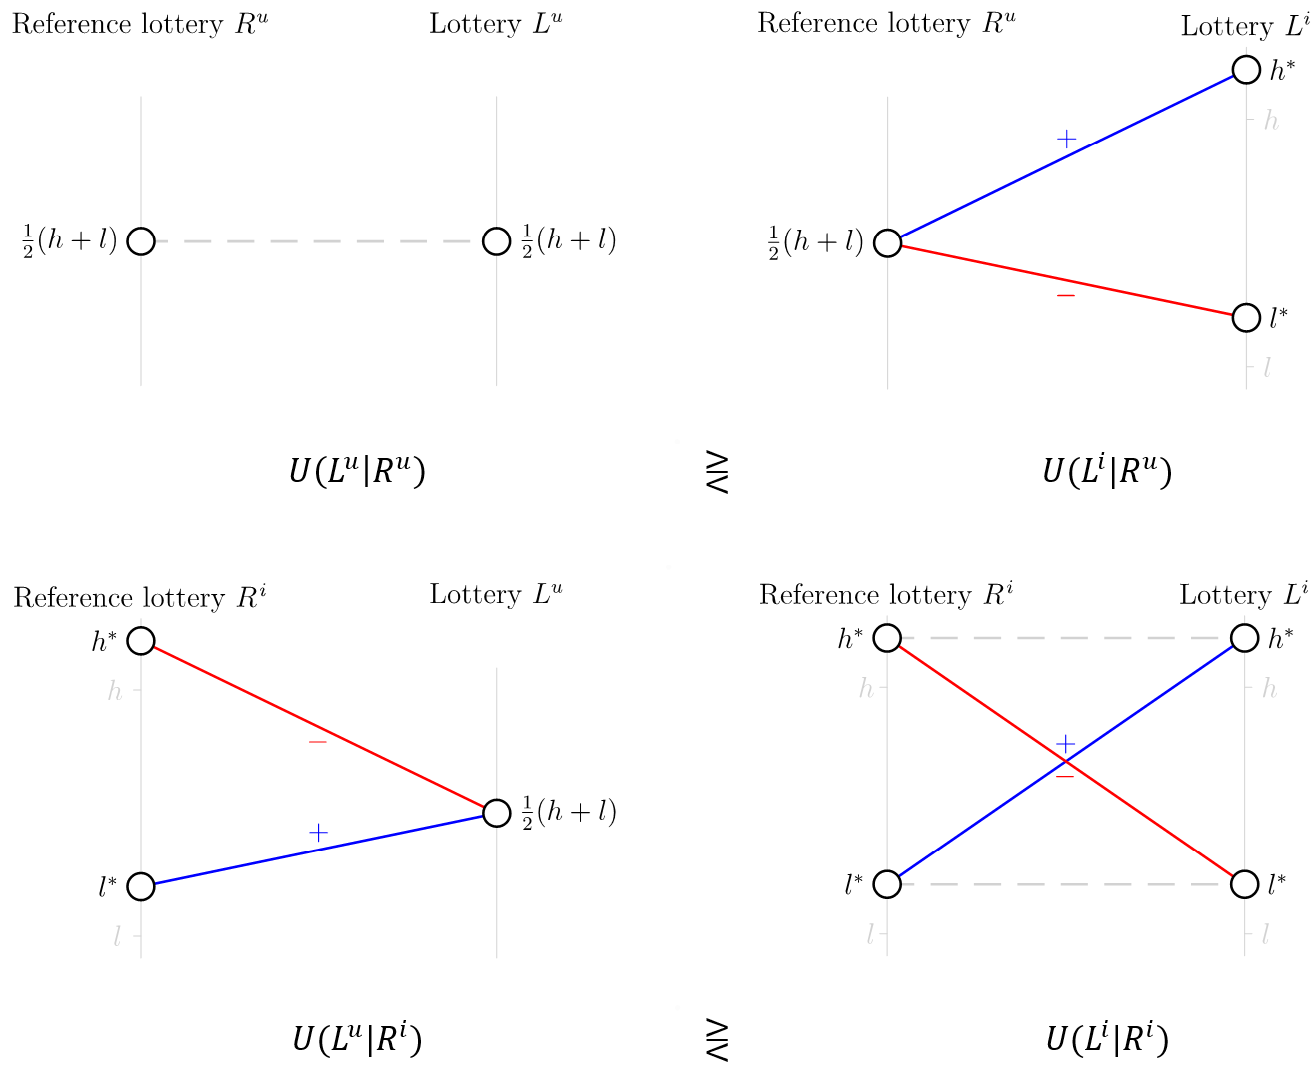
\includegraphics[width=1\textwidth]{./figures/theory_fig4.png}}
  \end{center}
\end{figure}

Figure \ref{fig:instrumental-KR} illustrates how the ability to adjust affects outcomes under the KR approach. As under the DA approach, it adds $0.5 \Delta + 0.5 \Delta = \Delta$ to the intrinsic utility of getting information, regardless of expectations. Also as under the DA approach, it adds $0.5 (1+\lambda) \Delta$ to gain-loss utility from getting unexpected information (the top-right panel), making the overall value of such information
\begin{equation*}
  U(L^i|R^u)-U(L^u|R^u)=-0.25(\lambda-1)(h-l)+\Delta+0.5(1+\lambda)\Delta.
\end{equation*}
Different from the DA approach, however, it enhances the value of \emph{not} getting expected information (the bottom-left panel) by an avoided loss of $\lambda \Delta$ only with probability one-half, toghether with a gain of $\Delta$ with probability one-half, resulting in the same addition of $0.5(1+\lambda)\Delta$ to gain-loss utility overall. Moreover, because both the $R^i$ and $L^i$ lotteries shift up by the same amount $\Delta$, gain loss utility from getting information (the bottom-right panel) is again unchanged. The overall value of expected information therefore becomes
\begin{equation*}
  U(L^i|R^i)-U(L^u|R^i)=-0.25(\lambda-1)(h-l)+\Delta+0.5(1+\lambda)\Delta,
\end{equation*}
which is identical to the value of unexpected information. The upshot is that the endowment effect $[U(L^i|R^i)-U(L^u|R^i)]-[U(L^i|R^u)-U(L^u|R^u)]$ stays the same: the implications of adjustments cancel out exactly.\footnote{Contrary to the result of Proposition \ref{prop:instrumental-DA}, this indifference result depends crucially on our simplifying assumption that adjustments to both the \enquote{good} and \enquote{bad} outcomes enhance utility by the same amount $\Delta$. More generally, if adjustments enhance the good outcome by $\Delta^h$ and the bad outcome by $\Delta^i \neq \Delta^h$, the endowment effect under the KR approach changes by $0.25(\lambda-1)(\Delta^h-\Delta^l) \neq 0$. Provided $\Delta^l<0.25(h-l)$, the overall endowment effect $0.25(\lambda-1)(h-l)+0.25(\lambda-1)(\Delta^h-\Delta^l)$ will remain positive.}

\FloatBarrier


% EXPERIMENTAL EVIDENCE --------------------------------------------------------
\section{Experimental evidence}

We used a laboratory experiment to test if preferences for information are reference dependent. A detailed description of procedures and participants is in Appendix \textbf{X}, and the complete experiment as seen by the participants is in online Appendix \textbf{X}.

\subsection{Experimental design}

\begin{figure}[ht]
  \caption{Structure of the experiment}\label{fig:expDesign}
  \begin{center}
  {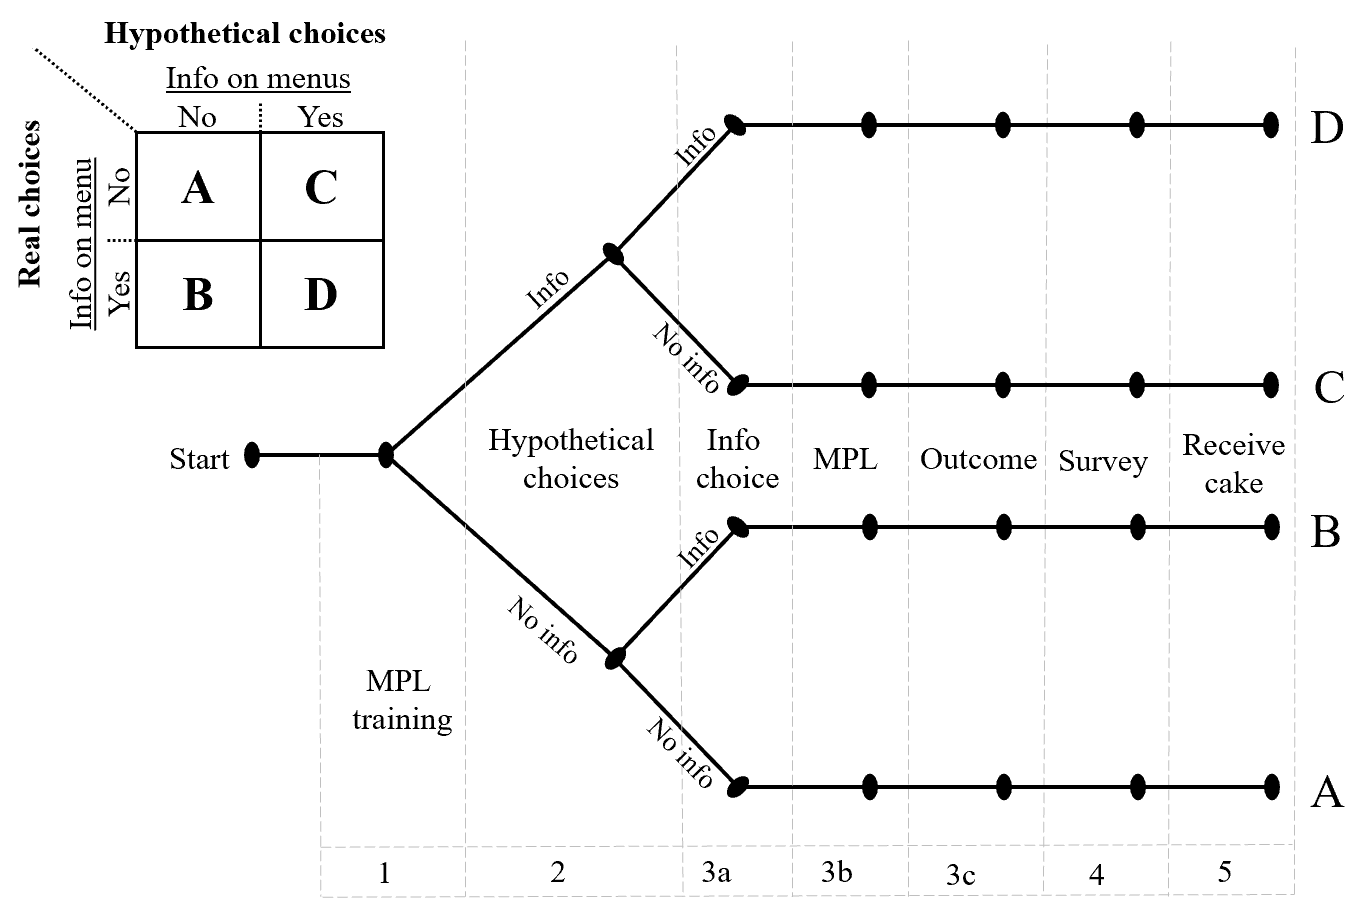
\includegraphics[width=1\textwidth]{./figures/experimentalDesign.png}}
  \end{center}
\end{figure}

Based on our recruitment flyer, all participants knew they would receive a cake for their participation in the experiment. After that, the experiment followed the structure shown in Figure \ref{fig:expDesign}. In step (1), we taught participants how to use a multiple-price list (MPL) and evaluated their understanding. In step (2), we asked participants to choose their preferred dessert from eleven consecutive dessert menus, each showing three desserts. These choices were not incentivized, and we were explicit about their hypothetical nature. In this step, we randomized half of the participants to see menus without calorie information and the other half to see menus with calorie information. The goal of this manipulation was to exercise some control over potential heterogeneity in expectations about information that participants might have brought to the laboratory. Making a series of choices from menus without (with) calorie information should set a baseline of low (high) expectations of receiving information when moving to the experiment’s next step.

In step (3a) participants were once again shown a menu with three desserts. One of these, a cake, was marked as the dessert they were about to actually receive, to eat after the experiment. Within each baseline group established in step (2), we again randomized participants into two groups, resulting in a $2 \times 2$ design. One group was \emph{endowed} with calorie information about the desserts, in the sense that the menu already showed a calorie-information column. The actual calorie numbers were \enquote{temporarily} \emph{xxx}-ed out, however, and participants in this group were asked whether they wanted to \enquote{keep} the calorie information, so they would see it, or \enquote{remove} the calorie information. The exact wording used is shown in \ref{fig:expManipulation} (top panel). The other group was \emph{not endowed} with calorie information, in the sense that the menu showed nothing calorie-related to begin with. Participants in this group were asked whether they wanted to \enquote{add} calorie information, so they would see it, or \enquote{keep} calorie information \enquote{off}. The exact wording used is shown in Figure  \ref{fig:expManipulation} (bottom panel).

\begin{figure}[ht]
  \caption{Key experimental manipulation}\label{fig:expManipulation}
  \begin{center}
  {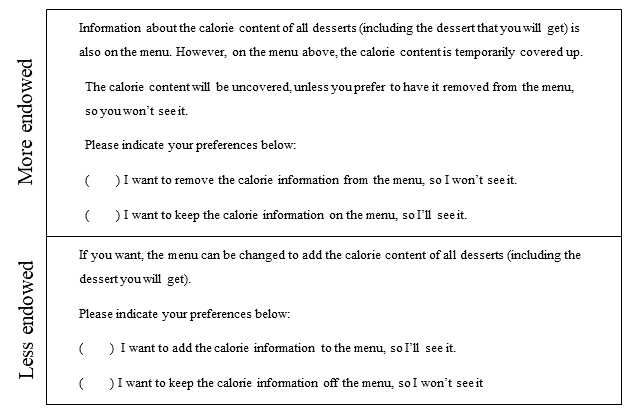
\includegraphics[width=1\textwidth]{./figures/keyManipulation.png}}
  \end{center}
\end{figure}

We argue that, compared to participants in the \emph{not endowed} treatment, participants in the \emph{endowed} treatment were more likely to expect to receive calorie information about their cake, for three reasons. First, the presence of \emph{xxx}-ed out calorie-information column on the menu was intended to make endowed participants focus first on getting calorie information when considering whether they want to actually see it, whereas the absence of any such information for non-endowed participants was intended to make them focus first on not getting it. Second, the menu description pointed to the calorie information as already being on the menu for endowed participants, but as needing a change in the menu for non-endowed participants. And third, the description of how participants could choose to see the information used \enquote{I want to keep} for endowed participants, but \enquote{I want to add} for non-endowed participants.

In step (3b) we aimed to elicit a monetary value for calorie information, using an MPL that allowed this value to range from negative to positive. For example, if participants chose to see the calorie information in step (3a), thereby indicating that information had positive value for them, we gave them the option to either keep the information on the menu (i.e., stick with their initial choice and ultimately see the information) or remove the information and receive some additional money. That is, we elicited their Willingness To Accept (WTA) to \emph{not} see the information after all. Conversely, if participants chose not to see the information in step (3a), thereby indicating that information had negative value for them, we elicited their WTA to \emph{see} the information after all, in a similar fashion.

The MPL included 10 choices, involving monetary amounts ranging from \$0.01 to \$5.00.\footnote{The complete list of values in the MPL is \$0.01, \$0.25, \$0.50, \$0.75, \$1.00, \$1.50, \$2.00, \$2.50, \$3.00, and \$5.00.}  Once all 10 choices were made, one choice was randomly selected to be binding.

In step (3c), participants were shown a menu on which the calorie information of the cake they were about to receive was either revealed or not, depending on the outcome of the MPL. In step (4), participants answered survey questions about their demographics, attitudes (risk preferences, time preferences, and degree of self-control), health status, health concern (the importance they assigned to their own health), and familiarity with calorie information (see \textbf{Appendix X} for a description of these data). Finally, in step (5), participants received their payment and cake.

\subsection{Identification strategy}

Based on our two consecutive manipulations to influence participants’ expectations about receiving calorie information, we organize participants in four groups: A, B, C, and D (see Figure \ref{fig:expDesign}). In the first manipulation, participants in groups A and B chose desserts from menus without calorie information, whereas participants in groups C and D chose desserts from menus with calorie information. In the second manipulation, participants in groups A and C chose whether to add information to a menu, whereas participants in groups B and D chose whether to keep information on a menu.

Because we are manipulating expectations, the timing and order of the manipulations matter. Specifically, for participants induced by the first manipulation to have high baseline expectations of receiving information (groups C and D), we expect the effect size of the second manipulation to be smaller. We therefore analyze that effect size separately for each baseline (i.e., groups A and B separately from groups C and D).

For each baseline, we identify the endowment effect by relating our experimental design to our theoretical definition of an endowment effect in equation \ref{eq:endowmentEffect}: $U(L^i|R^i)-U(L^u|R^i)>U(L^i|R^u)-U(L^u|R^u)$. For example, for participants induced by the first manipulation to have low baseline expectations of receiving information (groups A and B), being endowed with information in the second manipulation corresponds to having reference lottery $R^i$ (group B, left-hand side of the equation), while not being endowed corresponds to having reference lottery $R^u$ (group A, right-hand side of the equation). Within each group, choosing to receive information corresponds to choosing outcome lottery $L^i$, while choosing not to receive information corresponds to choosing outcome lottery $R^u$. Thus, we can infer whether $U(L^i|R^i)-U(L^u|R^i)$ is positive ($L^i$ is chosen) or negative for each participant in group B, and similarly infer whether $U(L^i|R^u)-U(L^u|R^u)$ is positive or negative for each participant in group A. Then, we aggregate the choices of each group and simply compare the share of participants in group A who chose to receive information to the share of participants in group B who did so. Furthermore, the heterogeneity in the data can be rationalized by assuming random utility.\footnote{Explicitly, participants could be heterogeneous in terms of self-control, curiosity, or concern about calorie intake.}

Our main goal is to show that preferences for information are not standard, and to propose that these preferences are reference-dependent. Therefore, we use the model of standard preferences as a straw man to set up null hypotheses to be rejected [CITE DELLAVEGINASPRENGER18]. Explicitly, we test the null hypothesis that the share of participants who choose to receive information is the same regardless of endowment status against the alternative that the share is higher for endowed participants. Note that the distinction between the DA approach and the KR approach does not play any role in the experiment: our design does not set out to distinguish between the two.\footnote{[CITE SPRENGER15] tests for the existence of an endowment effect for monetary risk using a design that does purposely distinguish between the DA and the KR approach. He shows that the data supports the KR approach instead of the DA approach.}

% RESULTS ----------------------------------------------------------------------
\section{Results}

We find evidence supporting the existence of an endowment effect for information: more participants chose to receive information when they were endowed with it, in the sense of getting a menu with temporarily \emph{xxx}-ed out calorie information. Furthermore, as expected, the effect was smaller for participants first primed to expect to receive information (i.e., participants who made initial hypothetical choices from menus with calorie information). A discussion of the empirical analysis and the results follows.

\subsection{Estimation strategy}

The goal of the analysis is to estimate the causal effect of receiving a menu with \emph{xxx}-ed out calorie information ($R^i$), relative to receiving a menu without \emph{xxx}-ed out calorie information ($R^u$), on the choice of receiving information ($L^i$) or not ($L^u$). Because we rely on the randomization process as identification strategy, unbiasedness of the unconditional ordinary least squares (OLS) estimator of the average treatment effect is guaranteed both under large- and finite-sample assumptions. However, the unbiasedness property guarantees only that the true treatment effect can be recovered by averaging the treatment effect over all potential realizations.\footnote{In general, the definition of a realization depends on the sources of uncertainty accounted for in the analysis. If only design-based uncertainty is considered, a realization is one draw of all possible randomizations within the population. If only sampling-based uncertainty is considered, a realization is one sample drawn from a superpopulation. Finally, if both sources of uncertainty are considered, a realization is a particular randomization from a particular sample [ABADIEETAL2020].} In practice, however, we get only one estimate of the treatment effect, obtained from the one realization we observe. This observed estimate reflects, in addition to the true treatment effect, any imbalances between treatment groups of variables that are prognostic (i.e., correlated with the dependent variable). For example, if by chance one treatment group ends up with 70\% rather than 50\% of the female participants, and if being female is prognostic, then the estimate of the treatment effect will be influenced by the gender imbalance.

Given that our sample size for estimating the treatment effect of the key experimental manipulation is about 110 participants, the estimate is likely to reflect covariate imbalances. Consequently, to address the uncertainty regarding the extent to which these imbalances matter, we present estimates from both the unconditional OLS estimator and from all possible conditional OLS estimators that can be created by adjusting the regression with all combinations of the set of prognostic covariates with large imbalances between groups.\footnote{There are no objective criteria to define \emph{large}. The term is subjective and roughly means \enquote{large enough to affect the treatment effect in an economically significant way.} We describe the method used to identify the set of covariates with large imbalances in \textbf{Appendix 3.}} Under large-sample assumptions, both the unconditional and the conditional estimators are unbiased. However, because the correlation between a covariate and the treatment variable might be different from zero, the conditional estimators present in our analyses are biased under finite-sample assumptions.\footnote{There are at least two alternatives to avoid the trade-off between unbiasedness and adjustments for covariate imbalance.

Ex-ante, one can use a randomized block design to force balance in prognostic covariates [ATHEYIMBENS17]. However, this design requires a solid understanding of the covariates that are prognostic of information preferences, as well as baseline data with those prognostic covariates. For this study, it was not feasible to use a randomized block design, because we did not have the baseline data and we were not willing to compromise the incentivized choices in the experiment by asking survey questions up front.

Ex-post, if one can create binary covariates\textemdash from the original covariates\textemdash and they partition the population, the OLS estimator of the average treatment effect is unbiased when a full set of interactions is included ([LIN13]; [ATHEYIMBENS17]). This approach is not feasible for our study either because, even if we could create binary covariates that partition the population, we do not have enough observations to estimate the regression with a full set of interactions.
}

\subsection{Results using choice data}

We first present the results for participants not primed with calorie information (groups A and B). The share of these participants who chose to receive information was $71\%$ for those endowed with information vs. $52\%$ for those not endowed ($p=0.02$ from a t-test and $p=0.05$ from a Fisher’s exact test,  both one-sided).\footnote{We use Simon Heß’s Stata program ritest (RITEST) with 5000 random permutations and the coefficient of the treatment from an OLS regression as the test statistic for our Fisher’s exact tests [IMBENSRUBIN15].} Figure \ref{fig:resultsLowBaseline} shows the implied treatment effect of $0.19$ and its associated $p$-value from an unconditional OLS regression, as well as 255 estimates and associated $p$-values from all possible adjusted regressions that can be estimated using the eight covariates with large imbalances between treatment groups A and B.

\begin{figure}[ht]
  \caption{Estimates of the treatment effect for participants in the low baseline}\label{fig:resultsLowBaseline}
  \begin{center}
  {\includegraphics[width=1\textwidth]{./figures/resultsLowBaseline.png}}
  \end{center}
\end{figure}

Of these 256 point estimates, 100\% are higher than $0.10$, 96.5\% are higher than $0.15$, and 20.1\% are higher than $0.20$. In addition, 99.6\%, 82\%, and 0\% of the estimates are statistically significant at the standard $0.1$, $0.05$, and $0.01$ levels of significance. Overall, we interpret these results as strong evidence for the existence of an endowment effect for information.

Next, we present the results for participants primed with calorie information (groups C and D). The share of these participants who chose to receive information was 65.5\% for those endowed with information vs. 59.5\% for those not endowed ($p=0.27$ from a t-test and $p=0.34$ from a Fisher’s exact test, both one-sided). Figure \ref{fig:resultsHighBaseline} shows the implied treatment effect of $0.06$ and its associated $p$-value from an unconditional OLS regression, as well as 1,024 estimates and associated $p$-values from all possible adjusted regressions that can be estimated using the ten covariates with large imbalances between treatment groups C and D.

\begin{figure}[ht]
  \caption{Estimates of the treatment effect for participants in the high baseline}\label{fig:resultsHighBaseline}
  \begin{center}
  {\includegraphics[width=1\textwidth]{./figures/resultsHighBaseline.png}}
  \end{center}
\end{figure}

Of these 1,024 point-estimates, 100\% are higher than $0$, 99.8\% are higher than $0.05$, 86\% are higher than $0.10$, 19\% are higher than $0.15$, and none are higher than $0.20$. In addition, 63\%, 10.5\%, and 0\% of the estimates are statistically significant at the standard $0.1$, $0.05$, and $0.01$ levels of significance. Overall, we interpret these results also as support for existence of an endowment effect\textemdash only one of the 1,024 point estimates is smaller than $0.05$. However, the size of the endowment effect is smaller for the primed participants of groups C and D than for the unprimed participants of groups A and B.

\subsection{Results using WTA data}

Finally, we designed the experiment to gather WTA data (from the multiple-price list) as an alternative measure of preferences for information. That is, we planned to reproduce the analyses presented above using, instead of the binary choice whether to receive information as a discrete dependent variable, WTA as a continuous dependent variable. Ex post, however, we realized that our way of eliciting WTA may not keep the relevant reference lottery constant, which makes it a questionable measure of participants’ value of information. For example, a participant randomized to receive a menu with \emph{xxx}-ed out calorie information (the \emph{endowed} treatment) starts out with reference lottery $R^i$ and then chooses to either have the information revealed, corresponding to outcome lottery $L^i$, or taken off the menu, corresponding to outcome lottery $L^u$. From her choice, we obtain our binary measure of information preferences by inferring that $U(L^i|R^i)-U(L^u|R^i)$ is positive if $L^i$ is chosen, and negative if $L^u$ is chosen. If she chooses to receive information, we elicit her WTA to take the information off the menu after all. This WTA is plausibly a measure of the weakly positive utility $U(L^i|R^i)-U(L^u|R^i)$ that she forgoes by giving up information. If, however, she chooses to take the information off, we elicit her WTA to keep the information on after all, and have it be revealed. At that point, we lose control of her referent. Although the WTA measures the weakly positive utility $U(L^u|\cdot)-U(L^i|\cdot)$, it is unclear whether she still considers herself endowed with information, which would imply that her reference lottery when completing the multiple-price list is still $R^i$, or whether her initial choice to take the endowed information off the menu changes her reference lottery to $R^u$.

This lack of clarity reflects a broader gap in our understanding of the referent formation process. [KR06] simply assume that the reference point depends on expectations held \enquote{in the recent past}, rather than expectations held at the time of consumption. They add that
\begin{displayquote}
  This does not assume that beliefs are slow to adjust to new information \emph{or that people are unaware of the choices that they have just made}\textemdash but that preferences do not instantaneously change when beliefs do. When somebody finds out five minutes ahead of time that she will for sure not receive a long-expected \$100, she would presumably immediately adjust her expectations to the new situation, but she will still five minutes later assess not getting the money as a loss. (p.1141, emphasis added).
\end{displayquote}

Applied to our context, this assumption implies that a participant’s choice of a particular outcome lottery need not instantaneously change her reference lottery. That is, she may still, at least for a while, feel endowed with information even if she just chose to give it up, or feel not endowed with information even if she just chose to get it.\footnote{Experimental results reported by [HEFFETZ18] in fact suggest that reference points do not necessarily change to match beliefs even gradually, through the mere passage of time.  Instead, \enquote{some sense of internalization of, or getting used to, the new expectations} is required (p.5).}

Nevertheless, we cannot \emph{rule out} that a participant's choice to either receive or not receive information might have moved her referent before completing the multiple-price list. As a result, we cannot treat the difference in information values elicited through our multiple-price list for endowed and not endowed participants as an estimate of the endowment effect expressed in dollar terms. What we can say is that, if an endowment effect does in fact exist, then any movement of participants' referents with their choices will bias downwards the elicited difference in information valuations.

The reason is straightforward. Let $\Re^i$ denote the subset of endowed participants, and $\Re^u$ the subset of not endowed participants. If participants' choice did \emph{not} move their referents, then the endowment effect could be estimated as the average revealed value of information for endowed participants minus the average revealed value of information for not endowed participants:
\begin{equation*}
  \frac{\sum_{j \in \Re^i}[U_j(L_j^i|R_j^i)-U_j(L_j^u|R_j^i)]}
       {|\Re^i|}
  -
  \frac{\sum_{j \in \Re^u}[U_j(L_j^i|R_j^u)-U_j(L_j^u|R_j^u)]}
      {|\Re^u|}.
\end{equation*}

If, on the other hand, participants' choices did move their referents, then the first average would be \enquote{contaminated} by some terms $U_j(L_j^i|R_j^u)-U_j(L_j^u|R_j^u)$, and the second average by some terms $U_j(L_j^i|R_j^i)-U_j(L_j^u|R_j^i)$. Suppose now that an endowment effect in fact exists (as defined in Equation \ref{eq:endowmentEffect}). Any contamination of the kind described will then tend to \emph{lower} the first average, since the contaminated terms $U_j(L_j^i|R_j^u)-U_j(L_j^u|R_j^u)$ will tend to be lower than the terms $U_j(L_j^i|R_j^i)-U_j(L_j^u|R_j^i)$ that they replace in the summation. Conversely, contamination will tend to \emph{raise} the second average, since the contaminated terms $U_j(L_j^i|R_j^i)-U_j(L_j^u|R_j^i)$ will tend to be higher than the terms $U_j(L_j^i|R_j^u)-U_j(L_j^u|R_j^u)$ that they replace. The upshot is that contamination will tend to reduce the estimated endowment effect relative to its true value.


\begin{figure}[ht]
  \caption{Estimates of the treatment effect for participants in the low baseline (WTA data)}\label{fig:resultsLowBaselineWTA}
  \begin{center}
  {\includegraphics[width=1\textwidth]{./figures/resultsLowBaselineWTA.png}}
  \end{center}
\end{figure}





\begin{figure}[ht]
  \caption{Estimates of the treatment effect for participants in the high baseline (WTA data)}\label{fig:resultsHighBaselineWTA}
  \begin{center}
  {\includegraphics[width=1\textwidth]{./figures/resultsHighBaselineWTA.png}}
  \end{center}
\end{figure}








% CONCLUSION -------------------------------------------------------------------
\section{Conclusion}

% BEGING WORKING AREA \\\\\\\\\\\\\\\\\\\\\\\\\\\\\\\\\\\\\\\\\\\\\\\\\\\\\\\\\\

\textbf{PENDING [See Klaas' and Linda's comments]}

% END WORKING AREA \\\\\\\\\\\\\\\\\\\\\\\\\\\\\\\\\\\\\\\\\\\\\\\\\\\\\\\\\\\\\


\clearpage


% REFERENCES -------------------------------------------------------------------


\clearpage

% APPENDICES -------------------------------------------------------------------

\end{document}
